\chapter{Method}\label{chapter:first_real_chapter}
From a probabilistic point of view, semantic segmentation can be modelled as $p_\theta(x,y)$, where $x$ is a given (RGB-)image, and $y$ is the semantic label. However, in practice, there also exists $z$, the physical object of which $x$ is a view. Thus, we propose the probabilistic model to be $p_\theta(x,y,z)$, which can be rewritten as: $p_\theta(x,y,z)$ = $p_\theta(y|x,z) p_\theta(x|z) p_\theta(z)$.
\begin{itemize}
    \item $p_\theta(z)$; The generative process of the object.
    \item $p_\theta(x|z)$; The generative process of the observation of the object.
    \item $p_\theta(y|x,z)$; The generative process of the semantic meaning in the viewport of the observation.
\end{itemize}
Notice that the model $p_\theta(x|z) p_\theta(z)$ is equal to the VAE. We propose to first learn the generative model $p_\theta(x,z) = p_\theta(x|z) p_\theta(z)$, by learning the approximation of $p_\theta(x|z)$ and $p_\theta(z)$, using a VAE. After which we can use that learnt model to approximate the parameters of $p_\theta(y|x,z)$.

\section{Model}
We start by rewriting the log-likelihood of $p_\theta(x, y)$ as shown in Eq.~\ref{eq:p_x_y_rewrite}. As the KL-divergence is $\geq 0$, the rest of the equation is the lower bound. Notice that the rest contains the $\mathcal{L}_ELBO$, which can be separated. This results in the equation $\mathcal{L}_{l-ELBO}$, shown in Eq.~\ref{eq:label_ELBO}. To be able to exert more control over the importance of each of the factors during training, we also introduce the $\mathcal{L}_{\beta\gamma l-ELBO}$, as shown in Eq.~\ref{eq:beta_label}.

\begin{subequations}
    \begin{align}
        \log p_\theta(x, y)
         & = D_{KL}(q_\phi(z|x) || p_\theta(z|x)) + \mathbb{E}_{q_{\phi}(z | x)}[\log p_\theta(x, y | z)] - D_{KL}(q_{\phi}(z|x) || p(z))  \label{eq:p_x_y_rewrite}                                                \\
         & \geq \mathbb{E}_{q_{\phi}(z | x)}[\log p_\theta(x, y | z)] - D_{KL}(q_{\phi}(z|x) || p(z))                                                                                                              \\
         & = \mathbb{E}_{q_{\phi}(z | x)}[\log p_\psi(y | x, z) + \log p(x | z)] - D_{KL}(q_{\phi}(z|x) || p(z))                                                                                                   \\
         & = \mathbb{E}_{q_{\phi}(z | x)}[\log p_\psi(y | x, z)] + \mathbb{E}_{q_{\phi}(z | x)}[\log p_\theta(x | z)] - D_{KL}(q_{\phi}(z|x) || p_\theta(z))                                                       \\
         & = \mathbb{E}_{q_{\phi}(z | x)}[\log p_\psi(y | x, z)] + \mathcal{L}_{ELBO}(\theta, \phi; x)                                                                                                             \\
         & = \mathcal{L}_{l-ELBO} \label{eq:label_ELBO}(\theta, \phi, \psi; x, z)                                                                                                                                  \\
        \mathcal{L}_{\beta\gamma l-ELBO}
         & = \mathbb{E}_{q_{\phi}(z | x)}[\log p_\psi(y | x, z)] + \gamma \cdot \mathbb{E}_{q_{\phi}(z | x)}[\log p_\theta(x | z)] - \beta \cdot D_{KL}(q_{\phi}(z|x) || p_\theta(z))        \label{eq:beta_label}
    \end{align}
\end{subequations}

Hence, we want to estimate the following three distributions using a neural network.
\begin{itemize}
    \item $q_\phi(z|x)$ (i.e. image encoder)
    \item $p_\theta(x|z)$ (i.e. image decoder)
    \item $p_\psi(y|x, z)$ (i.e. label decoder)
\end{itemize}
We will refer to the image encoder and label decoder together as VAE-Segmentation (VAES). A schematic of the model can be seen in Figure~\ref{fig:schematic-vaes}.

\begin{figure}[h]
    \centering
    \subfloat[A classic VAE and our model during the pre-training phase.\label{fig:schematic-vae}]{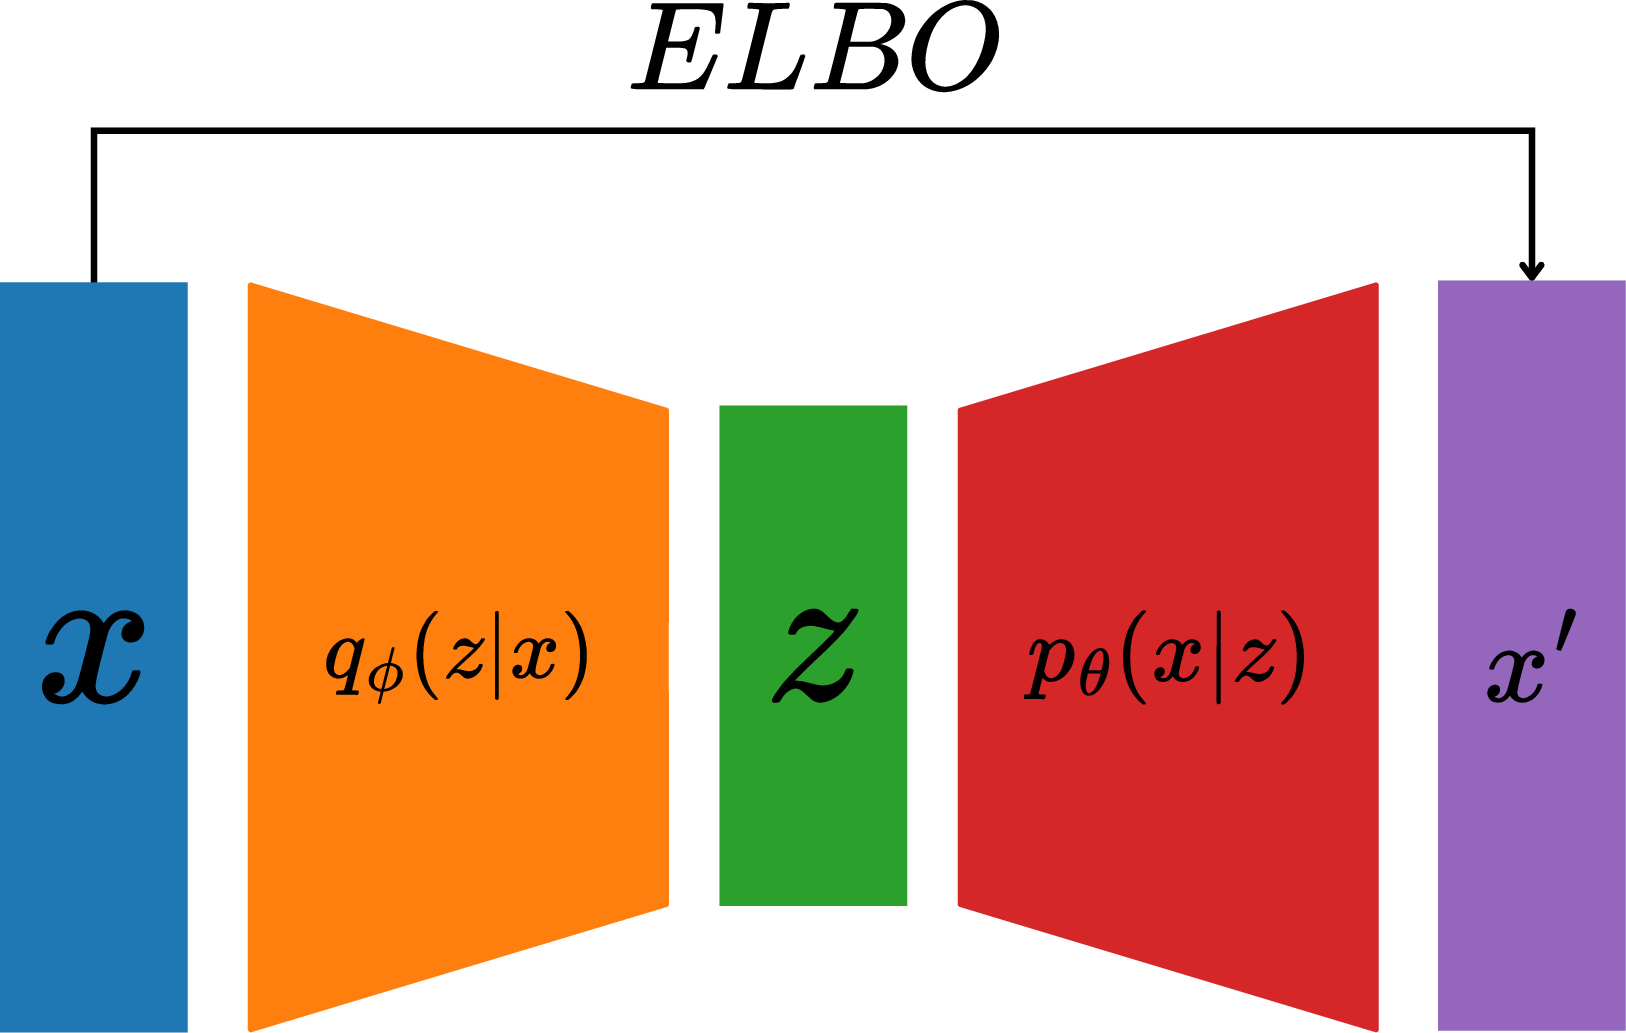
\includegraphics[width=0.45\textwidth]{figures/vae.png}}\hphantom{space}
    \subfloat[The full VAES model. The dotted line shows the skip connections. During inference the image decoder can be disregarded\label{fig:schematic-vaes}]{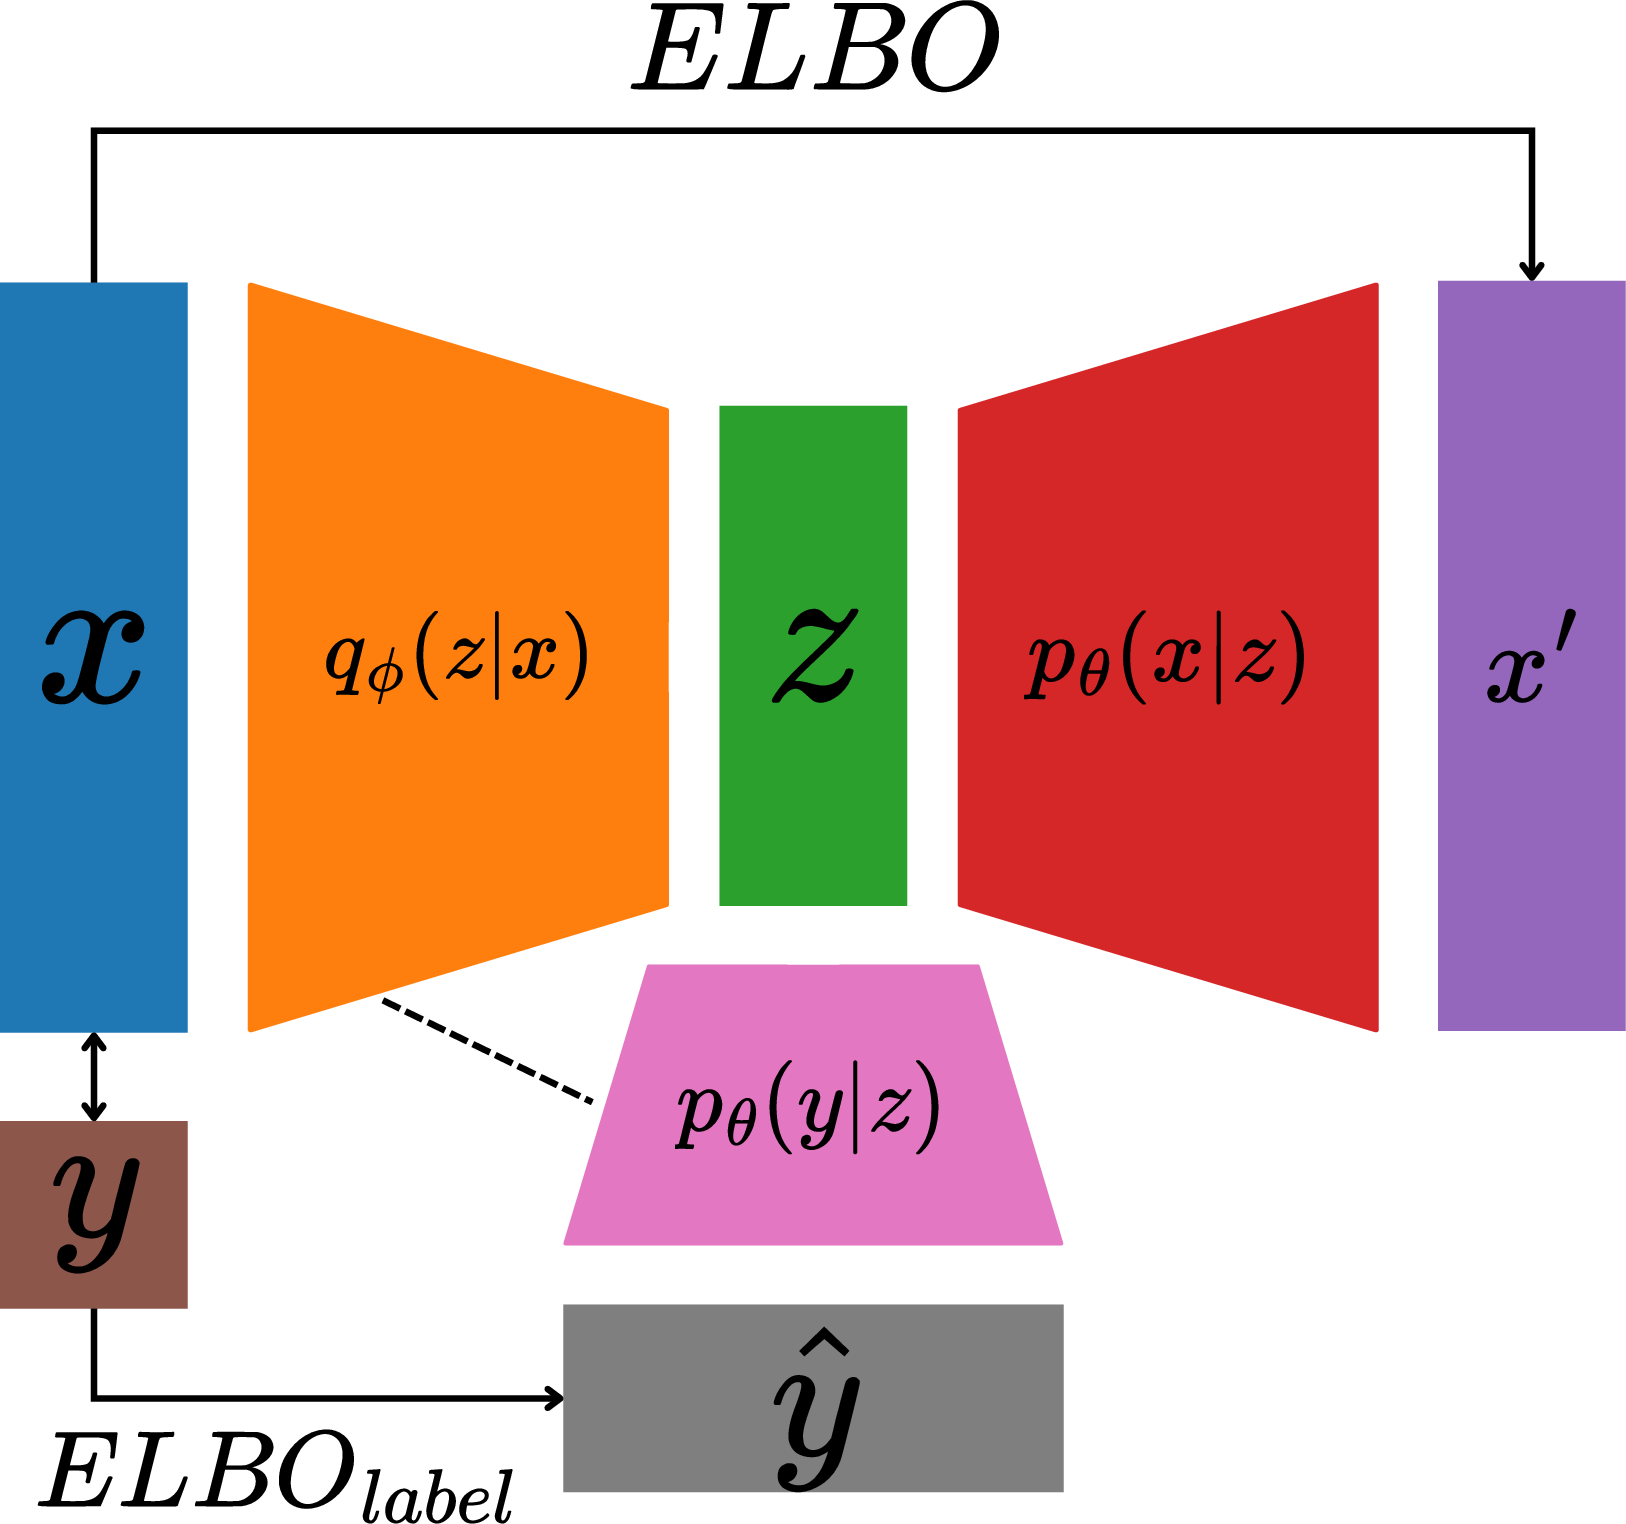
\includegraphics[width=0.45\textwidth]{figures/vaes.png}}
    \caption{A schematic of the proposed VAES.}
\end{figure}

\subsection{Image Encoder}
The image encoder approximates the latent distribution, $p_\theta(z)$. To ensure we can train the encoder using gradient descent, we need to make sure it is fully differentiable. Thus, we make use of the reparametrization trick. We use a deterministic mapping $g_\phi(\epsilon, z')$, where $\epsilon$ is an independent random variable and $g_\phi(x)$ is our (deterministic) neural network. Kingma et al.~\cite{kingma2014autoencodingvariationalbayes} show that by using this reparametrization trick a wide range of distributions can be learnt. In our case, we use a Gaussian latent space. The reparametrization then becomes $z = \mu + \sigma \epsilon$, where $\mu$ and $\sigma$ are the output of our image encoder network.

\subsection{Image Decoder}
The image decoder approximates the conditional Gaussian distribution $p_\theta(x|z)$. It is used during the pre-training step to prime the image encoder with 'good' initial weights, using the traditional ($\beta$-)VAE training. The hypothesis is, that given that $x$ can be reconstructed from the learnt $q_\phi(z|x)$, the learnt latent space contains useful features to approximate $p_\theta(y|x,z)$. In Eq.~\ref{eq:beta-elbo} $\log p_\theta(x|z)$ can be calculated using Eq.~\ref{eq:log_p_x_z} using a parameterized neural network.

\begin{equation}
    \begin{split}
        \log p_\theta(x|z)      & = \log \mathcal{N}(x; \mu, \sigma^2I) \label{eq:log_p_x_z} \\
        \text{where}~\mu,\sigma & =NN_\theta(z)
    \end{split}
\end{equation}

\subsection{Label Decoder}
The label decoder is similar to the image decoder, except that it approximates a multivariate Bernoulli distribution, instead of a Gaussian distribution. Thus, the calculation of $\log p_\theta(y|x,z)$ is different, which is shown in Eq.~\ref{eq:log_p_y_z}. Furthermore, it has `skip connections'. These skip connections allow for information to flow directly from a higher layer in the encoder to the decoder. We make the distinction between 3 types of skip connections.
\begin{enumerate}
    \item Skip. The output of the encoder layer is directly passed to the decoder.
    \item Projection. The output of the encoder layer is first projected using a convolutional layer.
    \item Variational. The output of the encoder layer is first projected using a variational convolutional layer.
\end{enumerate}
When all skip connections are of the type `Skip', our architecture is equal to the U-Net architecture.

\begin{subequations}
    \begin{align}
        \log p_\psi(y|x, z) & = \sum_{i=0}^n y_i \log h_i + (1 - y_i)\log(1-h_i) \label{eq:log_p_y_z} \\
        \text{where}~h      & = \text{softmax}(NN_\theta(x, z))
    \end{align}
\end{subequations}

\section{Training procedure}
The training consists of two stages, the pre-training phase, and the fine-tuning stage. 
\paragraph*{Pre-training phase} During the pre-training phase, the image encoder, $q_\phi(z|x)$, and image decoder, $p_\theta(x|z)$, are trained according to Algorithm~\ref{alg:pre-training}. This algorithm is equal to the one proposed by Kingma et al.~\cite{kingma2014autoencodingvariationalbayes}. The model parts shown in Figure~\ref{fig:schematic-vae} are optimized.

\RestyleAlgo{ruled}
\begin{algorithm}
    \caption{Pre-training: The pre-training phase is equal to the AEVB, i.e. VAE, algorithm proposed by Kingma et al.~\cite{kingma2014autoencodingvariationalbayes}.}
    $\theta, \phi \gets$ Initialize parameters\;
    \Repeat{Convergence of $\theta, \phi$}{
        $\mathbf{X}^M \gets $ Sample a random minibatch of size $M$\;
        $g \gets \nabla_{\theta, \phi} \mathcal{L}_{ELBO} (\theta, \phi; \mathbf{X}^M)$ Calculate the gradients.\; 
        $\theta, \phi \gets$ Update parameters using gradients $g$ (E.g. using AdaMax\cite{kingma2017adammethodstochasticoptimization}) \;
    }
    \Return{$\theta, \phi$}
    \label{alg:pre-training}
\end{algorithm}


\paragraph*{Fine-tuning phase} During the fine-tuning phase, the learnt image encoder, $q_\phi(z|x)$, is reused. A new label decoder, $p_\psi(y|x, z)$, is initialized and optimized. The encoder can either be jointly optimized or kept frozen. Note that if we are not interested in the probability $p_\phi(x | z)$ and have chosen $\gamma = 0$ for $\mathcal{L}_{\beta\gamma l-ELBO}$, we can disregard it to reduce the computational load during training. The pseudocode can be seen in Algorithm~\ref{alg:fine-tuning}.

\begin{algorithm}
    \caption{Fine-tuning: The fine-tuning phase }
    $\theta, \phi \gets$ Initialize $\theta, \phi$ using the pre-training algorithm shown in Algorithm~\ref{alg:pre-training}\;
    $\psi \gets$ Initialize $\psi$\;
    \Repeat{Convergence of $\psi, \phi$}{
        $\mathbf{X}^M, \mathbf{Y}^M \gets $ Sample a random minibatch of size $M$\;
        $z^M \sim q_\phi(z | \mathbf{X}^M)$ Sample from the learnt encoder\;
        $g \gets \nabla_{\psi, \phi} \mathcal{L}_{l-ELBO} (\psi, \phi; \mathbf{X}^M, z^M)$ Calculate the gradients\;
        $\psi \gets$ Update $\psi$ using gradients $g$ (E.g. using AdaMax~\cite{kingma2017adammethodstochasticoptimization})\;
        \lIf{$\theta$ is not frozen}{$\theta \gets$ Update $\theta$ using gradients}
        \lIf{$\gamma \neq 0$}{$\phi \gets$ Update $\phi$ using gradients}
    }
    \Return{$\psi, \phi$}
    \label{alg:fine-tuning}
\end{algorithm}


\section{Evaluation}
\subsection{Inference}
Due to the variational architecture of the model, the inference can be done in two ways. One way is deterministic, by taking the mode of each latent vector. The other is variational, by sampling each latent vector. During training sampling the latent space is useful to improve the stability of training. However, during evaluation, it is preferred for the model to be deterministic. Hence, during evaluation, the mode of the latent space is used.

\subsection{Metrics}
The most well-known and widely-used metrics within classification are precision (Eq.~\ref{eq:precision}), recall (Eq.~\ref{eq:recall}), and F1-score (Eq.~\ref{eq:f1})~\cite{rijsbergen1979information}. The latter is a combination of precision and recall. Within the field of image segmentation the F1-score is also sometimes referred to as the Recognition Quality (RQ). In this, TP, FP, and FN refer to the True Positive, False Positive, and False Negative predictions per pixel. As our model always gives a prediction for each pixel, an FP in one class will always coincide with an FN in another class. Another common metric is the Jaccard Index (Eq.~\ref{eq:jaccard}), which is monotonically similar to the F1-score but weighs incorrect predictions more. As they are similar we will only report the Jaccard Index.

\begin{subequations}
    \begin{align}
        \text{Precision}     & = \frac{TP}{TP + FP} \label{eq:precision}                                               \\
        \text{Recall}        & = \frac{TP}{TP + FN} \label{eq:recall}                                                  \\
        F1 = \text{RQ}       & = 2 \cdot \frac{\text{Precision} \cdot \text{Recall}}{\text{Precision} + \text{Recall}} \\ 
                             & = \frac{TP}{\frac{1}{2} (FN + FP) + TP} \label{eq:f1}                                   \\
        \text{Jaccard Index} & = \frac{TP}{FN + FP + TP} \label{eq:jaccard}
    \end{align}
\end{subequations}
